% LTeX: language=en-US
\documentclass[handout,usepdftitle=false,xcolor=dvipsnames,aspectratio=169]{beamer}
%\documentclass[beamer,usepdftitle=false,xcolor=dvipsnames,aspectratio=169]{beamer}
%\documentclass[trans,notes=show,usepdftitle=false,aspectratio=169]{beamer}


\usepackage[english]{babel}
\usepackage{iftex}
\ifPDFTeX
\usepackage[T1]{fontenc}
\usepackage[utf8]{inputenc}
\usepackage{lmodern}
\else
\usepackage{fontspec}
\defaultfontfeatures{Ligatures=TeX}
\setmainfont{Latin Modern Roman}
\setsansfont{Latin Modern Sans}
\setmonofont{Latin Modern Mono}
\usepackage{newunicodechar}
\newfontfamily\unicodeSymbolFont{Segoe UI Symbol}[
  BoldFont=Segoe UI Symbol,
  ItalicFont=Segoe UI Symbol,
  BoldItalicFont=Segoe UI Symbol
]
\newunicodechar{⟂}{{\unicodeSymbolFont ⟂}}
\fi
\usepackage{amsmath,amsfonts}
\usepackage{booktabs,multirow,xcolor,colortbl}
\usepackage{bm}%to use a more powerful version of \boldsymbol
\usepackage{fvextra}
\usepackage{csquotes}
\usepackage{textcomp}
\ifPDFTeX
\DeclareUnicodeCharacter{27C2}{\ensuremath{\perp}}
\fi

\newcommand{\AllSample}{ \mathcal Y^T }

\usepackage[citestyle=authoryear-comp,bibstyle=../Preamble/mystyle_lowercase,maxbibnames=5,minbibnames=1,maxnames=2, minnames=1,datezeros=false,date=long,isbn=false,url=false,backend=biber,useprefix=true]{biblatex}
\addglobalbib{../Preamble/Macro_database_biblatex.bib}	

\usepackage{upquote}
\usepackage{ragged2e}
\usepackage{microtype}

\usepackage{multimedia}
\usepackage{graphicx}
\usepackage[export]{adjustbox}
\usepackage{epstopdf}
\usepackage[labelfont=bf,format=hang, figurename=Fig.]{caption}
\usepackage[subrefformat=parens,labelformat=empty]{subcaption}
\usepackage{pgfpages} % for multiple-screen presentations

\usepackage{array}

\newcolumntype{L}[1]{>{\RaggedRight\let\newline\\\arraybackslash\hspace{0pt}}m{#1}}
\newcolumntype{C}[1]{>{\centering\let\newline\\\arraybackslash\hspace{0pt}}m{#1}}
\newcolumntype{R}[1]{>{\raggedleft\let\newline\\\arraybackslash\hspace{0pt}}m{#1}}
%https://tex.stackexchange.com/questions/12703/how-to-create-fixed-width-table-columns-with-text-raggedright-centered-raggedlef


%%% use serif font for math
\usefonttheme[onlymath]{serif}

%%% define blue highlighting
\newcommand{\highlight}[1]{{\color{blue}{#1}}}

%%%% define command for setting sources

\newcommand{\Source}{}

%%%
\beamertemplatenavigationsymbolsempty


%%% define themes
\usetheme{Boadilla}
\usecolortheme{rose}
\usecolortheme[named=blue]{structure}

\newcommand\textbox[1]{%
  \parbox{.333\textwidth}{#1}%
}

\setbeamertemplate{sections/subsections in toc}[sections numbered]


%%%% set coloring in  foot and head
\setbeamercolor{alerted text}{fg=red!80!black}
\setbeamertemplate{enumerate items}[default] % numbers enumerate items without encircling them
\setbeamertemplate{itemize items}[ball] % numbers enumerate items without encircling them
\setbeamercolor{section in head/foot}{fg=black, bg=white}
\setbeamercolor{subsection in head/foot}{fg=black, bg=white}
\setbeamercolor{title}{fg=black}
\setbeamercolor{subtitle}{fg=blue}

\setbeamertemplate{caption}[numbered]

%%% set overlays as default
\beamerdefaultoverlayspecification{<+->}

%%%% settings for output mode

\mode<beamer>
{
%\setbeameroption{show notes on second screen=right}
}

\mode<trans>
{\renewcommand{\highlight}[1]{{\textbf{#1}}}}


\mode<handout>
{
\renewcommand{\highlight}[1]{{\textbf{#1}}}
%\pgfpagesuselayout{4 on 1}[a4paper,border shrink = 5mm,landscape]
%\setbeamercolor{background canvas}{bg=black!5}
}


%%% define Exercise counter
\newcounter{Exercise}
\resetcounteronoverlays{Exercise}
\setcounter{Exercise}{0}
\newcommand{\Exercise}{\refstepcounter{Exercise}\emph{\structure{Übung \theExercise}: }}

%%%% define environments for theorems etc and make them numbered
\setbeamertemplate{theorems}[numbered]

\newtheorem{assum}{Assumption}
\setbeamertemplate{assum}[numbered]

\newtheorem{defin}{Definition}
\setbeamertemplate{defin}[numbered]

\newtheorem{propos}{Proposition}
\setbeamertemplate{propos}[numbered]


%%%% Make Parts show up in TOC
\makeatletter
\AtBeginPart{%
  \addtocontents{toc}{\protect\beamer@partintoc{\the\c@part}{\beamer@partnameshort}{\the\c@page}}%
}
%% number, shortname, page.
\providecommand\beamer@partintoc[3]{%
  \ifnum\c@tocdepth=-1\relax
    % requesting onlyparts.
    \makebox[6em]{#1.} #2
    \par
  \fi
}
\define@key{beamertoc}{onlyparts}[]{%
  \c@tocdepth=-1\relax
}
\makeatother%

%%%% fix bug in beamer package with note itemize
%%% http://tex.stackexchange.com/questions/1480/changing-the-textwidth-of-the-notes-in-beamer-repost-from-so
\makeatletter
\defbeamertemplate{note page}{infolines}
{%
  \vskip.75em
  \nointerlineskip
  \begin{minipage}{\textwidth} % this is an addition
  \footnotesize \insertnote
  \end{minipage}               % this is an addition
}
\makeatother

\setbeamertemplate{note page}[infolines]


\newcommand{\backupbegin}{
   \newcounter{framenumberappendix}
   \setcounter{framenumberappendix}{\value{framenumber}}
}
\newcommand{\backupend}{
   \addtocounter{framenumberappendix}{-\value{framenumber}}
   \addtocounter{framenumber}{\value{framenumberappendix}}
}

\hypersetup{bookmarksnumbered=true,naturalnames=true,pdfhighlight=/N,citebordercolor={1 1
1},linkbordercolor={1 1 1},colorlinks=true,anchorcolor=black,linkcolor=blue,citecolor=green,urlcolor=green,
pdfpagemode=UseOutlines,breaklinks=true,
pdfkeywords=Dynare, pdfsubject=Dynare,pdfstartpage=1} %pdfpagemode=fullpage

\usepackage[copyright]{ccicons}

\usepackage{tikz,pgfplots}
\pgfplotsset{compat=1.18}
\usetikzlibrary{arrows,calc,decorations.pathreplacing,decorations.shapes}
\pgfdeclarelayer{background}
\pgfdeclarelayer{foreground}
\pgfsetlayers{background,main,foreground}

\usepackage{relsize}
\newcommand\LM{\ensuremath{\mathit{LM}}}
\newcommand\IS{\ensuremath{\mathit{IS}}}
\DeclareMathOperator{\std}{std}


\setbeamertemplate{footline}{
\begin{beamercolorbox}{subsection in head/foot}
\insertsectionnavigationhorizontal{.95\textwidth}{\hskip0pt
\hfill}{\hfill \insertframenumber /\inserttotalframenumber}
\end{beamercolorbox}
}

\newenvironment{witemize}{\itemize\addtolength{\itemsep}{8pt}}{\enditemize}
\newenvironment{wenumerate}{\enumerate\addtolength{\itemsep}{8pt}}{\endenumerate}

\usepackage[]{minted}
\usepackage{tcolorbox}
\usepackage{etoolbox}
\BeforeBeginEnvironment{minted}{\begin{tcolorbox}[boxsep=0mm]}%
\AfterEndEnvironment{minted}{\end{tcolorbox}}%

\AtBeginEnvironment{minted}{%
  \renewcommand{\fcolorbox}[4][]{#4}}  


\title[]{\textbf{Advanced Dynare\\}
\medskip{Chapter II}\\
\emph{The Dynare preprocessor}
}

\author{Johannes Pfeifer}
\input{../date_place.txt}


\AtBeginSection[]
{
  \begin{frame}{Outline}
    \tableofcontents[currentsection]
  \end{frame}
    \begin{frame}
      \frametitle{Overview}
      \begin{center}
        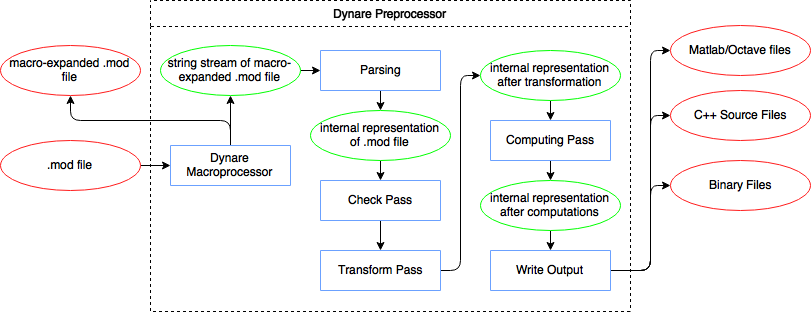
\includegraphics[width=13cm]{figures/overview.png}
      \end{center}
    \end{frame}
}

\begin{document}

\begin{frame}<4->
  \titlepage

  \begin{columns}[T]
    \column{0.3\textwidth}
    \column{0.09\textwidth}

     \ccbysa
    \column{0.61\textwidth}
    \tiny
    Copyright © 2007--2025 Dynare Team \\
    Licence: \href{http://creativecommons.org/licenses/by-sa/4.0/}{Creative
      Commons Attribution-ShareAlike 4.0}
  \end{columns}
\end{frame}

\begin{frame}
  \frametitle{Overview}
  \begin{center}
    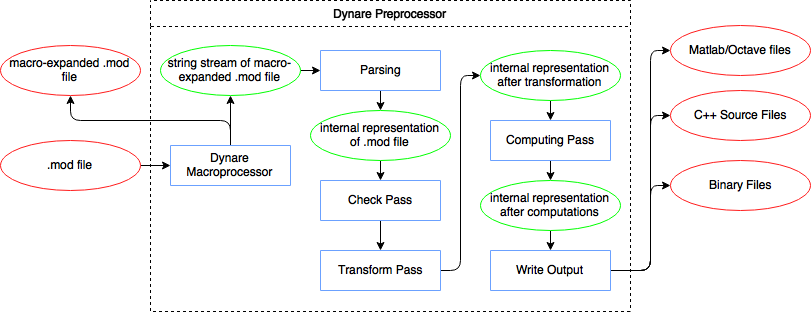
\includegraphics[width=13cm]{figures/overview.png}
  \end{center}
\end{frame}

\begin{frame}{Outline}
  \tableofcontents
\end{frame}

\section{Invoking the preprocessor}

\begin{frame}[fragile]
  \frametitle{Calling Dynare}
  \begin{witemize}
  \item Dynare is called from the host language platform with the syntax
      \begin{minted}{matlab}
    dynare FILENAME[.mod]
    \end{minted}
 \item This call can be followed by certain options:
    \begin{witemize}
    \item Some of these options impact host language platform functionality\\
    $\rightarrow$ \textit{e.g.} \texttt{nograph} prevents graphs from being displayed in MATLAB
    \item Some cause differences in the output created by default\\
    $\rightarrow$ \texttt{notmpterms} prevents temporary terms from being written to the static/dynamic files
    \item Others impact the functionality of the macroprocessor or the preprocessor\\
    $\rightarrow$ \textit{e.g.} \texttt{nostrict} shuts off certain checks that the preprocessor does by default
    \end{witemize}
    \begin{minted}{matlab}
    dynare FILENAME[.mod] nostrict
    \end{minted}

  \item Matlab command line supports syntax completion since Dynare 6.x
  \end{witemize}
\end{frame}

\begin{frame}[fragile]
  \frametitle{Command line options in the mod-file}
  \begin{witemize}
  \item Command line options can alternatively be defined in the first line of the .mod file
  \item Avoids to always have to invoke an option at the command line\\
  $\rightarrow$ particularly useful for the \texttt{nostrict} option during the development phase of a model
  \item Definition must be
  \begin{itemize}
    \item a one-line Dynare comment, i.e. begin //
    \item the options must be enclosed in \texttt{----+ options:} and \texttt{+----} and must be whitespace separated
    \item As in the command line, if an option admits a value, the equal symbol must not be surrounded by spaces
  \end{itemize}
    \begin{minted}{matlab}
    // --+ options: json=compute, stochastic, nostrict +--
    \end{minted}
  \end{witemize}
\end{frame}

\section{Macro processing}

\begin{frame}[fragile]
  \frametitle{Macro processing}
  \begin{witemize}
  \item The Dynare macro language provides a set of macro commands that can be used in \texttt{mod} files
  \item The macro processor employs text expansions/inclusions to transform a \texttt{mod} file with macro commands into a \texttt{mod} file without macro commands\\
  $\rightarrow$ result can be stored using \texttt{savemacro} option
  \item The result is fed to the parser\\
  $\rightarrow$ use \texttt{onlymacro} to stop after macro processing before parsing

    \begin{minted}{c++}
    dynare FILENAME[.mod] onlymacro savemacro=macroresult
    \end{minted}


  \item Attention: the macro processor only does text substitution; objects computed in later steps are not available yet and cannot be conditioned on for that reason
  \end{witemize}
\end{frame}


\section{Parsing}

\begin{frame}
\frametitle{Parsing overview}
\begin{witemize}
\item Parsing is the action of transforming an input text (a \texttt{mod} file in our case) into a data structure suitable for computation
\item The parser consists of three components:
  \begin{wenumerate}
  \item the \alert{lexical analyzer}, which recognizes the ``words'' of the \texttt{mod} file (analog to the \textit{vocabulary} of a language)
  \item the \alert{syntax analyzer}, which recognizes the ``sentences'' of the \texttt{mod} file (analog to the \textit{grammar} of a language)
  \item the \alert{parsing driver}, which coordinates the whole process and constructs the data structure using the results of the lexical and syntax analyses
  \end{wenumerate}
\end{witemize}
\end{frame}

\begin{frame}[fragile]
\frametitle{Undesired Parsing}
\begin{witemize}
  \item Dynare will try to parse all tokens it recognizes
  \item Code not recognized by the parser is directly passed to the preprocessor output\\
  $\rightarrow$ allows using MATLAB/Octave commands directly in the mod-file
  \item Causes problems when one wants to invoke commands containing recognized tokens
 \end{witemize}
\end{frame}

\begin{frame}[fragile]
\frametitle{Bypassing the parsing}
\begin{witemize}
  \item The \texttt{verbatim;} block instructs Dynare not to parse text contained in it
  \item In the following example, \texttt{stoch\_simul} would otherwise be recognized as a Dynare command during parsing
\end{witemize}
\begin{minted}{c++}
verbatim;
rhos = [ 0.8, 0.9, 1];
for iter = 1:length(rhos)
    set_param_value('rho',rhos(iter));
    [info, oo_, options_, M_] = stoch_simul(M_, options_, oo_, var_list_)
    if info(1)~=0
        error('Simulation failed for parameter draw')
    end
end
end;
  \end{minted}
\end{frame}


\begin{frame}
\frametitle{1.\ Lexical analysis}
\begin{witemize}
\item The lexical analyzer recognizes the ``words'' (or \alert{lexemes}) of the language
\item When invoked, the lexical analyzer reads the next characters of the input, tries to recognize a lexeme, and either produces an error or returns the associated token
\end{witemize}
\end{frame}

\begin{frame}
\frametitle{2.\ Syntax analysis}
\begin{witemize}
\item The \texttt{mod} file grammar is transformed into C++ source code by the program \texttt{bison}
\item The grammar tells a story which looks like:
  \begin{witemize}
  \item A \texttt{mod} file is a list of statements
  \item A statement can be a \texttt{var} statement, a \texttt{varexo} statement, a \texttt{model} block, an \texttt{initval} block, \ldots
  \item A \texttt{var} statement begins with the token \texttt{VAR}, then a list of \texttt{NAME}s, then a semicolon
  %\item A \texttt{model} block begins with the token \texttt{MODEL}, then a semicolon, then a list of equations separated by semicolons, then an \texttt{END} token
  %\item An equation can be either an expression, or an expression followed by an \texttt{EQUAL} token and another expression
  %\item An expression can be a \texttt{NAME}, or a \texttt{FLOAT\_NUMBER}, or an expression followed by a \texttt{PLUS} and another expression, \ldots
  \end{witemize}
\end{witemize}
\end{frame}

\begin{frame}[fragile]
\frametitle{Syntax analysis}
\begin{witemize}
\item Using the list of tokens produced by lexical analysis, the syntax analyzer determines which ``sentences'' are valid in the language, according to a \alert{grammar} composed of \alert{rules}.
\item \texttt{(1+3)*2; 4+5;} will pass the syntax analysis without error
\item \texttt{1++2;} will fail the syntax analysis, even though it has passed the lexical analysis
\end{witemize}
\end{frame}


\begin{frame}
\frametitle{3.\ Parsing driver}

\begin{witemize}
\item The parsing driver opens the \texttt{mod} file and launches the lexical and syntactic analyzers
\item It implements most of the semantic actions of the grammar\\
$\rightarrow$ creates data structure representing the \texttt{mod} file
\item If there is a parsing error
\begin{itemize}
    \item unknown keyword
    \item syntax errors
    \item use of undeclared symbols in model block, \texttt{initval} block\ldots
    \item use of a symbol incompatible with its type (\textit{e.g.} parameter in \texttt{initval}, local variable used both in model and outside model)
    \item \ldots
    %\item multiple shock declarations for the same variable
\end{itemize}
it displays the line and column numbers where the first error occurred and exits\\
$\rightarrow$ there may be others only displayed when the first error is fixed
\end{witemize}
\end{frame}

\section{Check pass}

\begin{frame}
  \frametitle{Check pass}
  \begin{witemize}
  \item Some errors in the \texttt{mod} file can be detected during parsing, but some other checks can only be done when parsing is completed\ldots
  \item The check pass performs many checks. Examples include:
    \begin{witemize}
    \item check there is at least one equation in the model (except if doing a standalone BVAR estimation)
    \item checks for coherence in statements (\textit{e.g.} options passed to statements do not conflict with each other, required options have been passed)
    \item checks for coherence among statements (\textit{e.g.} if \texttt{osr} statement is present, ensure \texttt{osr\_params} and \texttt{optim\_weights} or \texttt{planner\_objective} statements are present (and not both))
    \item checks for coherence between statements and attributes of \texttt{mod} file (\textit{e.g.} \texttt{use\_dll} is not used with \texttt{block} or \texttt{bytecode})
    \end{witemize}
  \end{witemize}
\end{frame}

\section{Transform pass}

\begin{frame}
  \frametitle{Transform pass (1/2)}
  \begin{witemize}
  \item The transform pass makes necessary transformations to prepare the \texttt{ModFile} object for the computing pass. Examples of transformations include:
    \begin{witemize}
    \item creation of auxiliary variables and equations for leads, lags, expectation operator, differentiated forward variables, etc.\\
        $\rightarrow$ more information stored in \texttt{M\_.aux\_vars} and at \href{https://git.dynare.org/Dynare/dynare/-/wikis/Auxiliary-variables}{Wiki}
    \item detrending of model equations if nonstationary variables are present
    \item decreasing leads/lags of \texttt{predetermined\_variables} by one period
    \item addition of FOCs of Lagrangian for \texttt{ramsey\_model}
    \item setup of OccBin structure
    \item addition of \texttt{dsge\_prior\_weight} initialization before all other statements if estimating a DSGE-VAR where the weight of the DSGE prior of the VAR is calibrated
    \end{witemize}
  \end{witemize}
\end{frame}

\begin{frame}
  \frametitle{Transform pass (2/2)}
  \begin{witemize}
  \item Finally, checks are performed on the transformed model
  \item Examples include:
    \begin{witemize}
    \item same number of endogenous variables as equations (not done in certain situations, \textit{e.g.} \texttt{ramsey\_model}, \texttt{discretionary\ policy}, where checks are done in Matlab)
    \item correspondence among variables and statements, \textit{e.g.} Ramsey, identification, perfect foresight solver, and perfect foresight solver are incompatible with \texttt{var\_exo\_det}
    \item correspondence among statements, \textit{e.g.} for DSGE-VAR with \texttt{bayesian\_irf} option, the number of shocks must be equal to the number of observed variables
    \end{witemize}
  \end{witemize}
\end{frame}


\section{Computing pass}

\begin{frame}
  \frametitle{Overview of the computing pass}
  \begin{witemize}
  \item Computing pass creates static model from dynamic one (by removing leads/lags)
  \item Determines which derivatives to compute and computes:
    \begin{witemize}
    \item lead/lag variable incidence matrix
    \item symbolic derivatives w.r.t. endogenous, exogenous, and parameters, if needed
    \item equation normalization + block decomposition
    \item temporary terms
    %\item computes equation cross references, if desired
    \end{witemize}
  \item Asserts that equations declared linear are indeed linear (by checking that Hessian == 0)
  \end{witemize}
\end{frame}

\begin{frame}
  \frametitle{Variables in the dynamic model}
  \begin{witemize}
  \item \texttt{Dynamic Model} is characterized by leag/lag incidence matrix stored in\\ \texttt{M\_.lead\_lag\_incidence}:
    \begin{itemize}
    \item \texttt{max\_lag + max\_lead + 1} rows (usually 3): the first row indicates $t-1$ (if applicable), the second row $t$, and the third row $t+1$ (if applicable)
    \item one column for every endogenous symbol in order of declaration\\
    $\rightarrow$ includes endogenous and exogenous auxiliary variables created during the transform pass
    \item elements of the matrix are either 0 (if the variable does not appear in the model) or correspond to the variable's column in the Jacobian of the dynamic model
    \end{itemize}
  \end{witemize}
    \center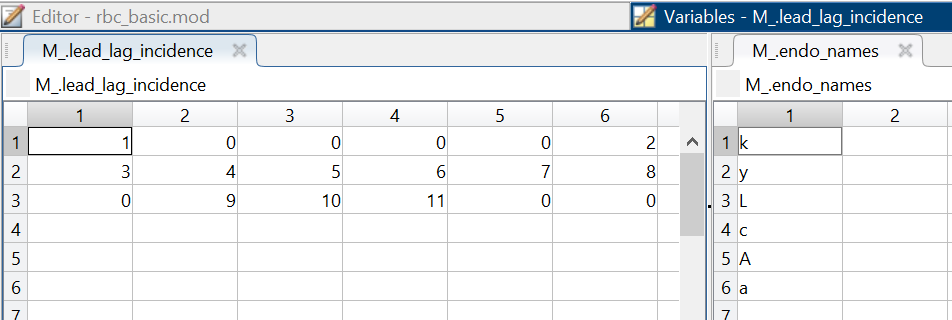
\includegraphics[width=9cm]{figures/lead_lag_incidence.png}
\end{frame}

\begin{frame}
  \frametitle{Static versus dynamic model}
  \begin{witemize}
  \item The static model is simply the dynamic model without leads and lags, used to characterize the steady state
  \item The Jacobian of the static model is used in the (MATLAB) solver for determining the steady state
  \end{witemize}
  \begin{block}{Example}
    \begin{witemize}
    \item suppose dynamic model is $2x_t \cdot x_{t-1} = 0$
    \item static model is $2x^2 = 0$, whose derivative w.r.t. $x$ is $4x$
    \item dynamic derivative w.r.t. $x_t$ is $2x_{t-1}$, and w.r.t. $x_{t-1}$ is $2x_t$
    \item removing leads/lags from dynamic derivatives and summing over the two partial derivatives w.r.t. $x_t$ and $x_{t-1}$ gives $4x$
    \end{witemize}
  \end{block}
\end{frame}

\begin{frame}
  \frametitle{Which derivatives to compute?}
  \begin{witemize}
  \item In deterministic mode:
    \begin{itemize}
    \item static Jacobian w.r.t. endogenous variables only
    \item dynamic Jacobian w.r.t. endogenous variables only
    \end{itemize}
  \item In stochastic mode:
    \begin{witemize}
    \item static Jacobian w.r.t. endogenous variables only
    \item dynamic Jacobian w.r.t. endogenous, exogenous, and deterministic exogenous variables
    \item dynamic Hessian w.r.t. endogenous, exogenous, and deterministic exogenous variables
    \item possibly dynamic 3rd derivatives (if \texttt{order} option $\geq 3$)
    \item possibly dynamic Jacobian and/or Hessian w.r.t. parameters (if \texttt{identification} or \texttt{analytic\_derivation} needed for \texttt{estimation} and \texttt{params\_derivs\_order} $>0$)
    \end{witemize}
  \item For Ramsey policy: the same as above, but with one further order of derivation than declared by the user with \texttt{order} option
  \end{witemize}
\end{frame}

\begin{frame}[fragile]
  \frametitle{Temporary terms (1/2)}
  \begin{itemize}
  \item When the preprocessor writes equations and derivatives in its outputs, it takes advantage of sub-expression sharing
  \item In MATLAB static and dynamic output files, equations are preceded by a list of \highlight{temporary terms}
  \item These terms are variables containing expressions shared by several equations or derivatives\\
  $\rightarrow$ greatly enhances the computing speed of the model residual, Jacobian, Hessian, or third derivative
  \end{itemize}
  \begin{columns}<.->
\begin{column}[T]{0.5\textwidth}
Original:
\begin{minted}{c++}
residual(0)=x+y^2-z^3;
residual(1)=3*(x+y^2)+1;
\end{minted}
\end{column}
\begin{column}[T]{0.5\textwidth}
Optimized:
\begin{minted}{c++}
T1=x+y^2;
residual(0)=T1-z^3;
residual(1)=3*T1+1;
\end{minted}
\end{column}
\end{columns}
\end{frame}

\begin{frame}
  \frametitle{Temporary terms (2/2)}
  \begin{witemize}
  \item Expression storage in the preprocessor implements maximal sharing, but this is not optimal for the MATLAB output files, because creating a temporary variable also has a cost (in terms of CPU and of memory)
  \item Computation of temporary terms implements a trade-off between:
    \begin{witemize}
    \item cost of duplicating sub-expressions
    \item cost of creating new variables
    \end{witemize}
  \item Algorithm uses recursive cost calculation that marks some nodes as being ``temporary''
  \item \textit{Problem}: redundant with optimizations done by the C/C++ compiler (when Dynare is in DLL mode)\\
   $\Rightarrow$ compilation very slow on big models
  \end{witemize}
\end{frame}

\section{Writing outputs}

\begin{frame}
  \frametitle{Output overview}
  \begin{witemize}
  \item If \texttt{mod} file is \texttt{mymodel.mod}, all created files will be in a namespace \texttt{mymodel} (\texttt{+mymodel} subfolder)
  \item Main output file is \texttt{mymodel.driver}, containing:
    \begin{itemize}
    \item general initialization commands
    \item symbol table output (variable and parameters names etc. )
    \item lead/lag incidence matrix
    \item call to MATLAB functions corresponding to the statements of the \texttt{mod} file
    \end{itemize}
  \item Subsidiary output files:
    \begin{itemize}
    \item for the static model (residuals, temporary terms, derivatives)
    \item for the dynamic model (residuals, temporary terms, derivatives)
    \item one for the auxiliary variables in the dynamic model (if relevant)
    \item one for the steady state file (if relevant)
    \item for the planner objective and Lagrange multipliers (static residuals and derivatives, if relevant)
    \item one each for the static and dynamic parameter derivatives (if required)
    \end{itemize}
  \end{witemize}
\end{frame}

%\begin{frame}
%  \frametitle{Model output files}
%  Three possible output types:
%  \begin{itemize}
%  \item MATLAB/Octave mode: static and dynamic files in MATLAB
%  \item Julia mode: static and dynamic files in Julia
%  \item DLL mode:
%    \begin{itemize}
%    \item static and dynamic files in C++ source code (with corresponding headers)
%    \item compiled through \texttt{mex} to allow execution from within MATLAB
%    \end{itemize}
%  \item Sparse DLL mode:
%    \begin{itemize}
%    \item static file in MATLAB
%    \item two possibilities for dynamic file:
%      \begin{itemize}
%      \item by default, a C++ source file (with header) and a binary file, to be read from the C++ code
%      \item or, with \texttt{no\_compiler} option, a binary file in custom format, executed from MATLAB through \texttt{simulate} DLL
%      \item the second option serves to bypass compilation of C++ file which can be very slow
%      \end{itemize}
%    \end{itemize}
%  \end{itemize}
%\end{frame}

\end{document}
